Die Anforderungen an den Verstärker sind eine hohe Eingangsimpedanz damit das Signal nicht belastet wird und eine möglichst große Spannungsverstärkung nah am Detektor um ein optimales Signal zu Rausch Verhältnis zu gewährleisten.
Für den Verstärker wird die Schaltung wie sie in Abbildung \ref{fig:Amp} links dargestellt ist verwendet, Sourceschaltung\cite{Tietze2002} genannt.
In dieser Schaltung wird das Gate des HEMT $T$ als Eingang verwendet.
In das Gate fließt fast kein Strom daher wird der Eingangswiderstand als unendlich angesehen.
Wie bei FETs müss allerdings auch bei HEMTs die parasitären Gate-Drain und Gate-Source Kapazitäten berücksichtigt werden.
Da es sich bei der Sourceschaltung zusätzlich um einen invertierenden Verstärker handelt muss der Millereffekt berücksichtigt werden.
Dieser beschreibt die effektive Vergrößerung der Gate-Drain Kapazität aufgrund der Spannungsverstärkung $V_U$
\begin{equation}
C_M = (1+ |V_U|)C_{gd}.
\end{equation}
\begin{minipage}[!b]{\textwidth}
\begin{minipage}[c]{0.4\textwidth}
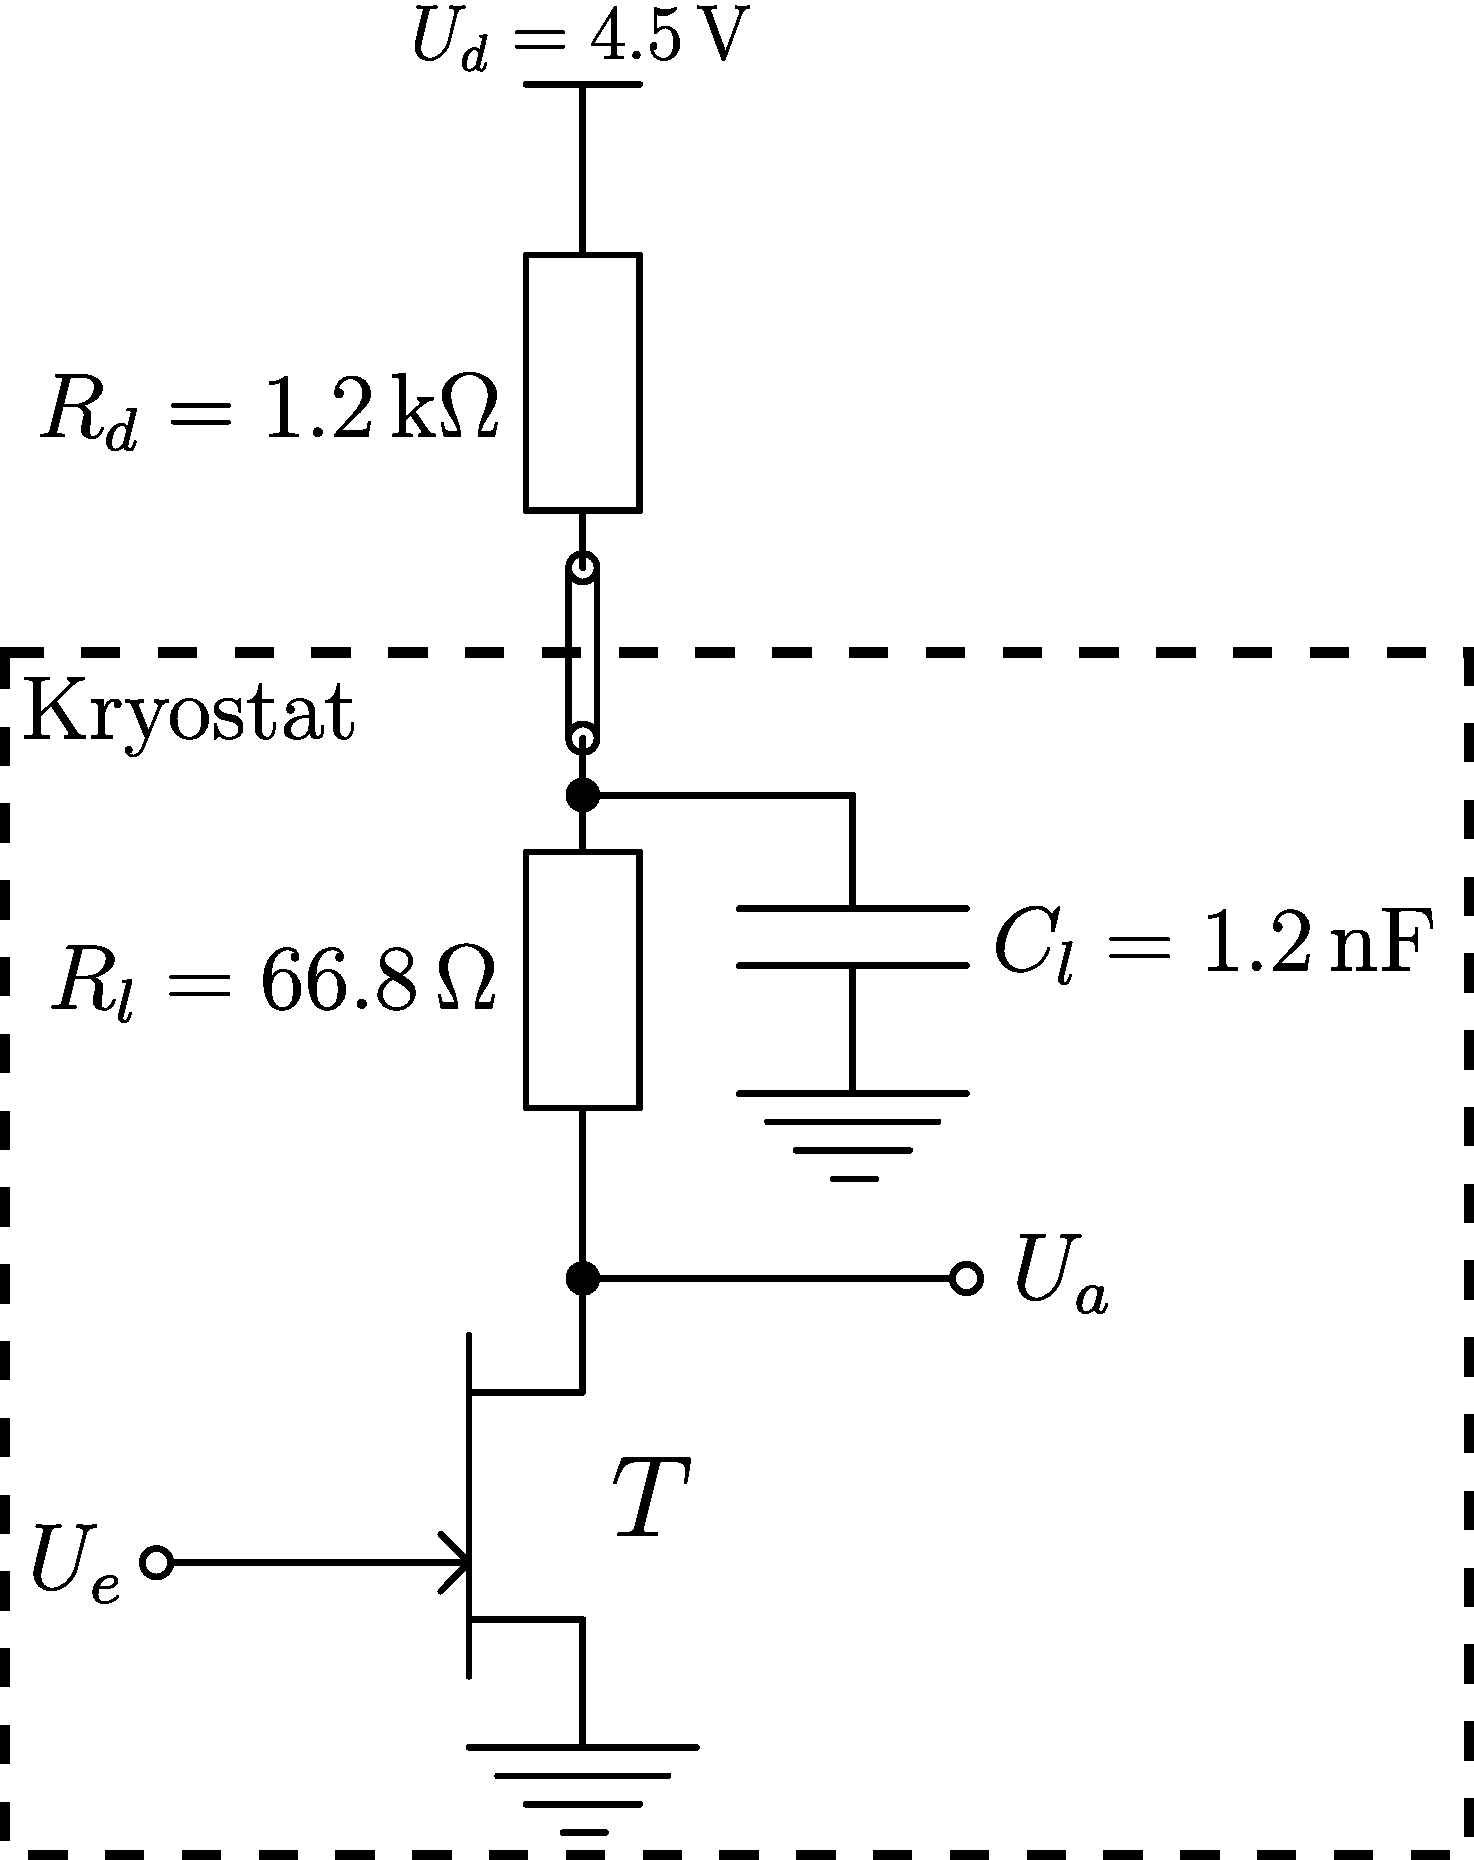
\includegraphics[width=0.9\textwidth]{./fig/Amp.pdf}
\end{minipage}
\begin{minipage}[c]{0.6\textwidth}
\begin{minipage}[c]{0.5\textwidth}
  \begin{tabular}{cc} \toprule
  Eingangskapazität & $\SI{127}{\pico\farad}$ \\ 
  Ausgangswiderstand ($\SI{10}{\kilo\hertz}$) & $\SI{1167}{\ohm}$ \\
  Transkonduktanz & $\SI{410}{\milli\siemens}$\\
  Grenzfrequenz Tiefpass & $\SI{1.99}{\mega\hertz}$\\
  Gate Leckstrom & $\sim\SI{1}{\micro\ampere}$ \\
  Leistung im Warmen &  $\SI{4.1}{\milli\watt}$\\
  Leistung im Kryostat &  $\SI{4.5}{\milli\watt}$\\ \bottomrule
 	\end{tabular}
\end{minipage} \\
\begin{minipage}[c]{0.5\textwidth}
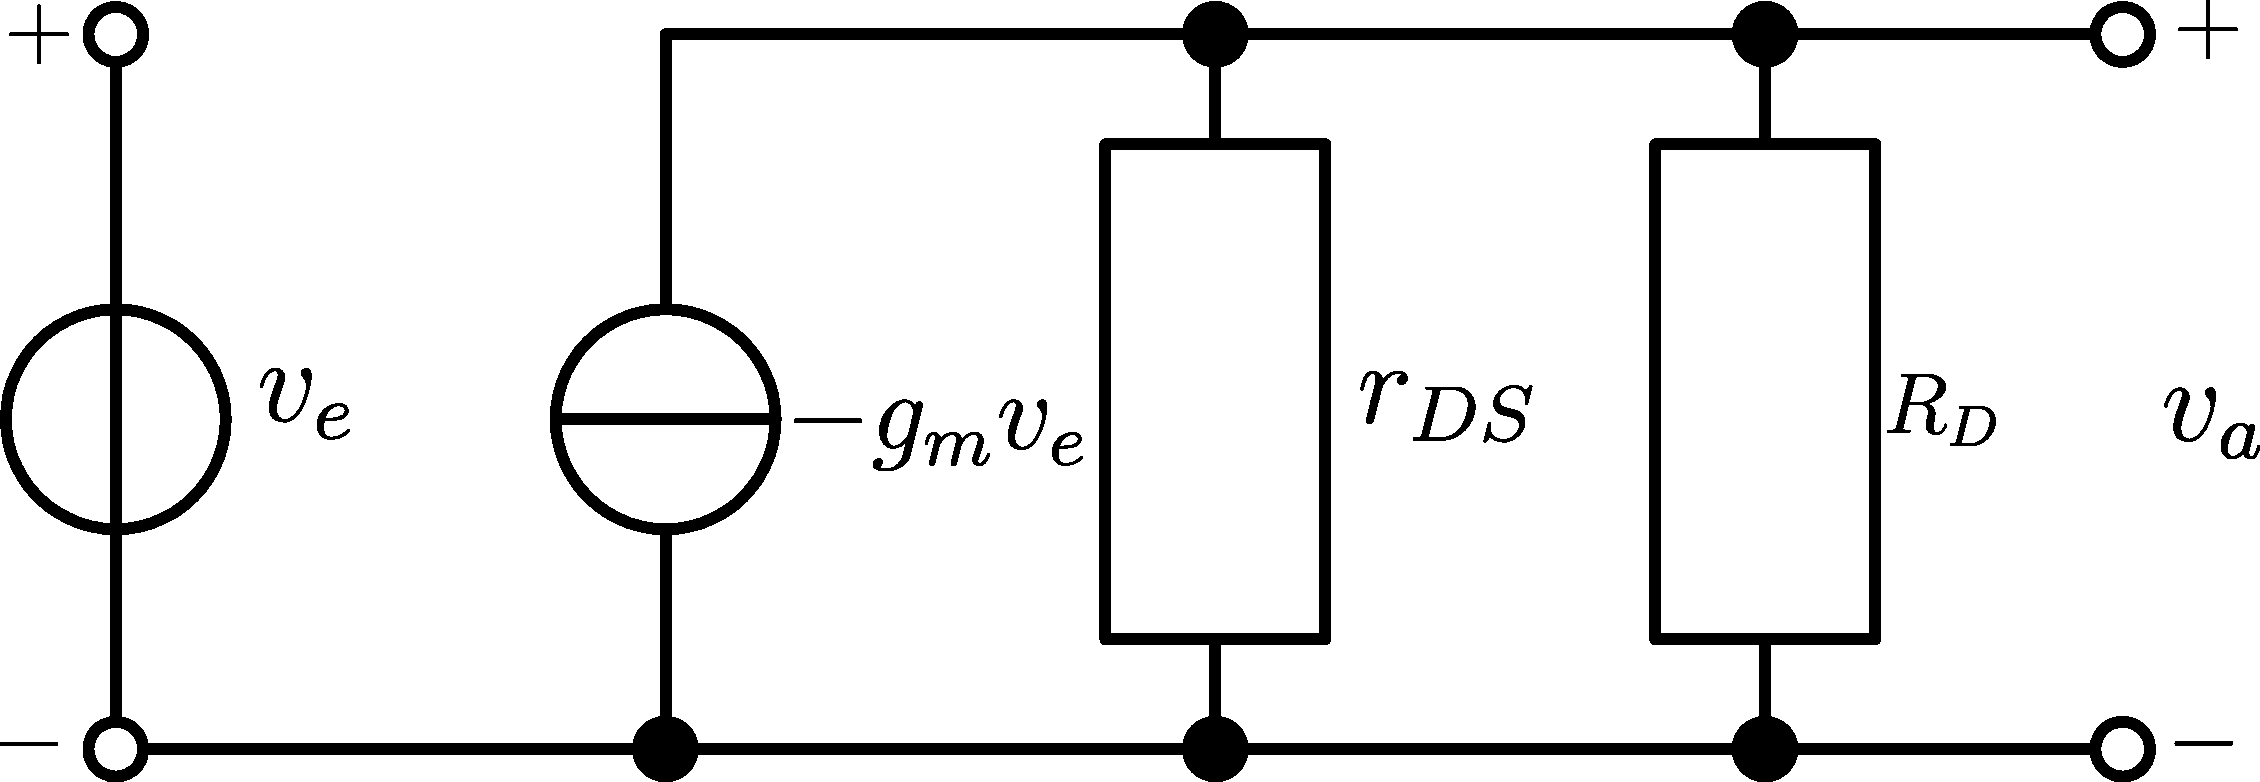
\includegraphics[width=2\textwidth]{./fig/AmpEq.pdf}
\end{minipage}
\end{minipage}
\captionof{figure}{Links: Schaltbild des Verstärkers mit Aufteilung in Raumtemperatur und Kryostat Anteil. Rechts oben: Wichtige Parameter berechnet aus den Angaben im Datenblatt zu dem handelsüblichen HEMT ATF-54143\cite{ATF-54143}. Rechts unten: Ersatzschaltbild des links dargestellten Verstärkers.}
\label{fig:Amp}
\end{minipage}
\vspace{1mm}
Für die Eingangskapazität gilt also $C_e = C_{gs} + C_M$.

Das Ersatzschaltbild ist in Abbildung \ref{fig:Amp} rechts unten dargestellt.
Der Transistor wird durch eine spannungsgesteuerte Stromquelle ersetzt.
Dieser wandelt die Eingangspannung mittels der Transkonduktanz $g_m$ in einen dazu proportionalen Strom.
Für die Spannungsverstärkung ergibt sich
\begin{equation}
V_U = \frac{v_a}{v_e} = -\frac{(r_{DS}||R_D)g_mv_e}{v_e} = -(r_{DS}||R_D)g_m \approx
-g_m R_D.
\end{equation}
Der Widerstand $R_D$ ist eine Kombination aus den Widerständen und Kapazitäten $R_d$, $R_l$, $C_l$ und daher Frequenzabhängig.
In dem interessanten Bereich $\text{DC} \-- \SI{10}{\kilo\hertz}$ ist er allerdings nahezu konstant.
\begin{equation}
R_D = R_l + \frac{R_d}{1 + 2\pi R_d C_l f} \approx R_l + R_d
\end{equation}
Die Verstärkung hängt somit entscheidend von der Transkonduktanz, welche in der Regel stark Temperaturabhängig ist, und dem Drainwiderstand $R_D$ ab.
Um die Abhängigkeit der Verstärkung von der Transkonduktanz und dadurch von der Temperatur aufzuheben wird oftmals ein teil des Ausgangssignal auf den Eingang rückgekoppelt.
Auf kosten einer kleineren Verstärkung wird diese dadurch stabilisiert.
Aufgrund der nur sehr kleinen Temperaturschwankungen im Kryostaten ist dies hier nicht notwendig und birgt eher das Risiko, dass der Verstärker anfängt zu schwingen.
Durch das vergrößern des Widerstand $R_D$ kann die Verstärkung nicht beliebig groß gewählt werden, da man sonst an den Rand des Ausgangskennlinienfeld gerät, d.h. am Transistor fällt eine zu kleiner Spannung ab und es fließt ein zu kleiner Strom.

Der Ausgangswiderstand ist gegeben durch
\begin{equation}
R_a = \frac{u_a}{i_a} = r_{DS}||R_D \approx R_D.
\end{equation}
Der Großteil des Drainwiderstand ist außerhalb des Kryostat dadurch wird die Leistung welche innerhalb des Kryostaten verbraucht wird minimiert.
Die Leistung spielt eine entscheidende Rolle dabei wie viele Detektoren im Kryostaten betrieben werden können.

Die Kombination aus $R_l$ und $C_l$ bildet zusammen einen Tiefpass mit der Grenzfrequenz
\begin{equation}
f_{-3\,\mathrm{db}} = \frac{1}{2\pi R_l C_l}
\end{equation}
Dadurch bleibt der interessante Frequenzbereich unbeeinflusst aber es wird verhindert, dass hochfrequente Schwingungen über die Kabel zurück auf den Eingang des Verstärkers koppeln.
Die Größe der Grenzfrequenz ist durch die verfügbaren Kapazitäten und durch die Leistung welche im Kryostat verbraucht werden soll begrenzt.

